\begin{frame}
\frametitle{Training}
\begin{enumerate}
\item Effect of payoff function
\item Effect of time
\item Effect of algorithm
\item Playing with oneself
\item Training with existing models
\end{enumerate}
\end{frame}

%%%

\begin{frame}
\frametitle{Effect of payoff function}

\begin{columns}[t]

\begin{column}{.5\textwidth}
\begin{figure}
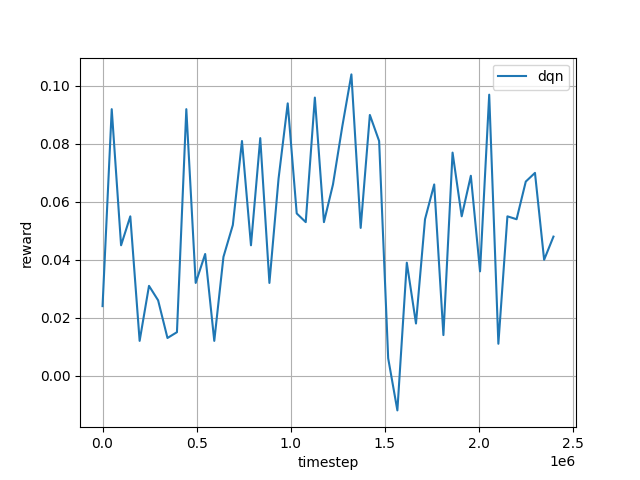
\includegraphics[height=.5\textheight]{dqn-no-specific-payoff.png}
\caption{DQN: win or lose}
\end{figure}
\end{column}

\begin{column}{.5\textwidth}
\begin{figure}
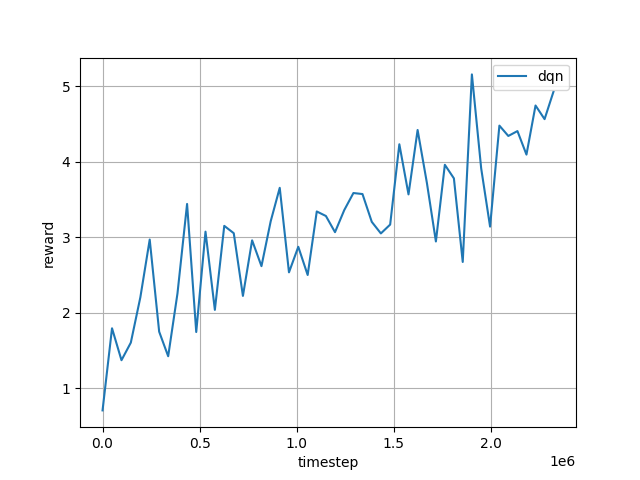
\includegraphics[height=.5\textheight]{dqn-specific-payoff.png}
\caption{DQN: count points}
\end{figure}
\end{column}

\end{columns}

\begin{itemize}
\item Deep-Q Learning, $t = \numprint{2500000}$, random agents
\item Average payoff stagnates or increases
\item Quality of payoff function determines success
\end{itemize}
\end{frame}

%%%

\begin{frame}
\frametitle{Effect of time}

\begin{columns}[c]

\begin{column}{.5\textwidth}
\begin{figure}
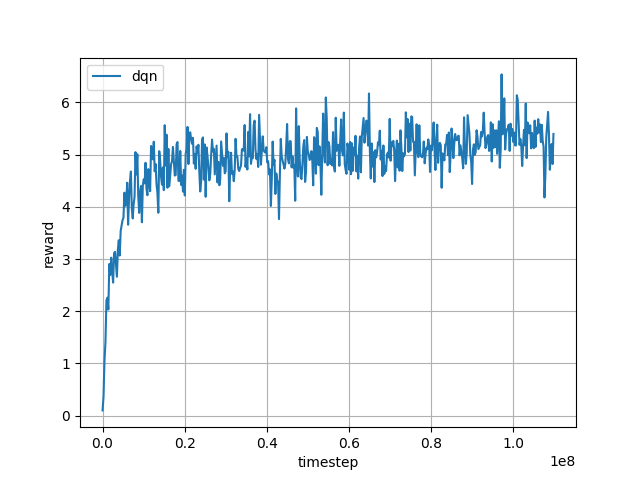
\includegraphics[width=\textwidth]{dqn_custom-payoff_result_long-run.png}
\caption{DQN: count points}
\end{figure}
\end{column}

\begin{column}{.5\textwidth}
\begin{itemize}
\item Deep-Q Learning, $t = \numprint{100000000}$, random agent
\item Reward at global maximum after \numprint{20000000} steps
\item Longer training will not lead to better results per se
\end{itemize}
\end{column}

\end{columns}

\end{frame}

%%%

\begin{frame}
\frametitle{Effect of algorithm}

\begin{columns}[t]

\begin{column}{.5\textwidth}
\begin{figure}

\includegraphics[height=.5\textheight]{nfsp.png}
\caption{NFSP: win or lose}
\end{figure}
\end{column}

\begin{column}{.5\textwidth}
\begin{figure}
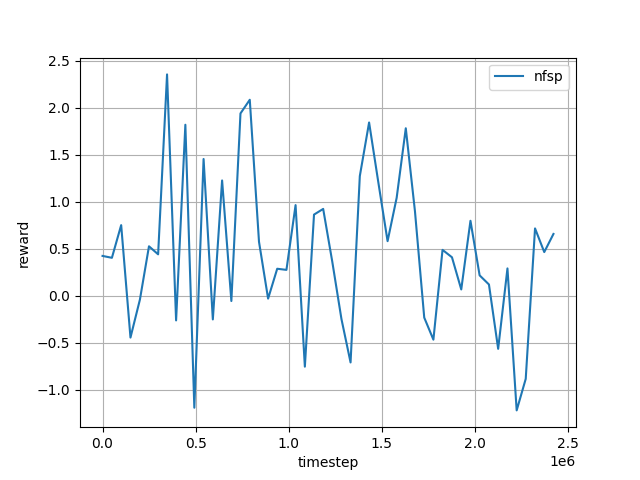
\includegraphics[height=.5\textheight]{nfsp-custom-payoff.png}
\caption{NFSP: count points}
\end{figure}
\end{column}

\end{columns}

\begin{itemize}
\item Neural Fictitious Self-Play, $t = \numprint{2350000}$, random agents
\item Regardless of the payoff function the AI can not beat a random player
\end{itemize}
\end{frame}

%%%

\begin{frame}
\frametitle{Playing with oneself}
\begin{columns}[c]

\begin{column}{.5\textwidth}
\begin{itemize}
\item Deep-Q Learning, $t = \numprint{2000000}$, experienced DQN agent
\item Only slightly better average payoff, even after \numprint{8000000} steps
\item DQN agents do not seem to improve iteratively
\end{itemize}
\end{column}

\begin{column}{.5\textwidth}
\begin{figure}
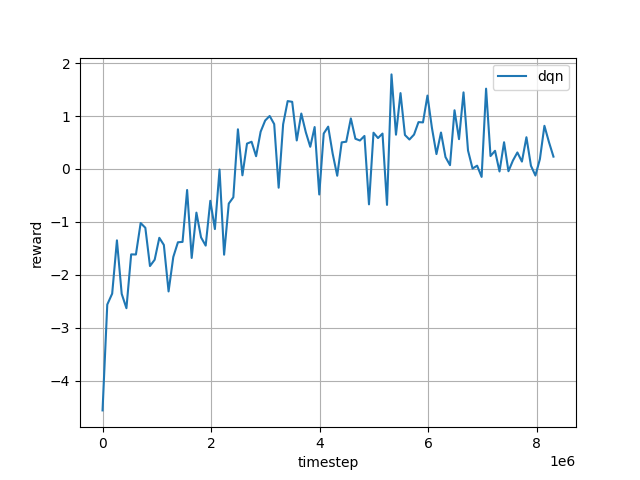
\includegraphics[width=\textwidth]{dqn_vs_dqn_long.png}
\caption{DQN vs DQN: count points}
\end{figure}
\end{column}

\end{columns}
\end{frame}

%%%

\begin{frame}
\frametitle{Training with existing models}
\begin{columns}[c]

\begin{column}{.5\textwidth}
\begin{figure}
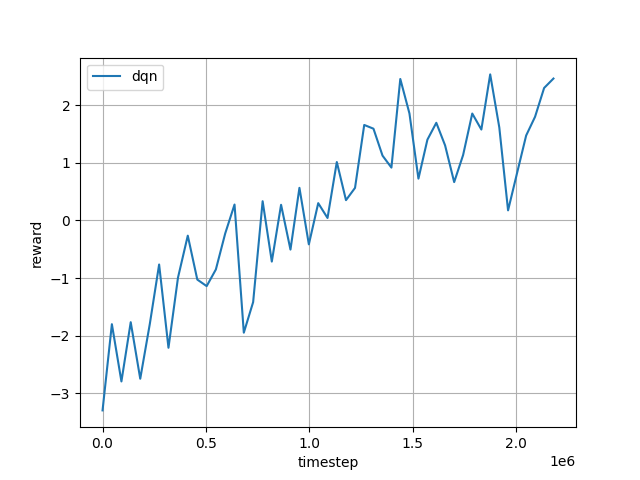
\includegraphics[width=\textwidth]{dqn_vs_dmc_5000_2000.png}
\caption{DQN vs DMC}
\end{figure}
\end{column}

\begin{column}{.5\textwidth}
\begin{itemize}
\item Deep-Q Learning, $t = \numprint{1000000}$, Deep Monte-Carlo agent
\item Beats adversary after \numprint{1000000} time steps
\item Eventually achieves a slightly better average payoff
\end{itemize}
\end{column}

\end{columns}
\end{frame}